\section{Einführung}
\begin{frame}{}
\begin{center}
    {\Huge Ich habe keine Antworten!}\\
    Aber ich helfe euch die richtigen Fragen zu stellen.

\end{center}
\end{frame}

\begin{frame}{Ich}
    \begin{table}
        \begin{tabularx}{\textwidth}{rll}
            bis 2013 & Schule & \\            
            & & \\
            2013 - 2020 & Studium der Physik & Mechanik\\
            & Uni Bonn & Thermodynamik\\
            & & Quantenmechanik\\
            & & Programmieren\\
            & & Elektronik\\
            & & \\
            Seit 2020 & Doktorand & Signalverarbeitung\\
            & Forschungszentrum Jülich & Teilchendetektoren\\
            & & Integrierte Schaltungen\\  
            & & Wissenschaftliches Schreiben \\
            & & Präsentieren \\
        \end{tabularx}
    \end{table}
\end{frame}

%\begin{frame}{Worüber rede ich?}
%\tableofcontents[sectionstyle=show,subsectionstyle=show/hide]
%\end{frame}

\subsection{Anforderungen von Studenten}
\begin{frame}{Übersicht}
Was sind klassische Arbeiten eines Studenten?
    \begin{itemize}
        \item Mitschreiben 
        \item Aufgaben bearbeiten
        \item Quellen sichten
        \item Arbeiten schreiben
        \item Präsentieren
        \item Kollaborieren\pause
        \item[$\Rightarrow$] Wissen ansammeln und teilen  \pause
        \item[$\Rightarrow$] \sout{Wissen} Daten ansammeln und teilen   
    \end{itemize}
\end{frame}
\note{Welche Art von arbeiten erledigen studenten regelmäßig?
Am Ende dient alles dem lernen, dem erlangen von Wissen!
Wissen ist auch nur eine Art von Daten!}

\begin{frame}{Wie hab ich es gemacht?}
    \begin{tabularx}{\linewidth}{ll}
        Mitschriften & Papier, Tablet \\
        Abgaben, Übungen & Papier\\
        Hausarbeiten, Thesis & \LaTeX\\
        Präsentationen & Powerpoint, \LaTeX\\
        Kommunikation & WhatsApp\\
        Teilen von Unterlagen & Dropbox (später Sciebo)\\                
    \end{tabularx}
    \pause
    \begin{tikzpicture}[overlay, remember picture]
        \node[anchor=south east] at ([shift={(-2.5cm,4cm)}]current page.south east) {
\includegraphics[width=3cm]{graphics/Meine_Mitschriften.jpg}};
        \pause
        \node[anchor=south east] at ([shift={(-2cm,3cm)}]current page.south east) {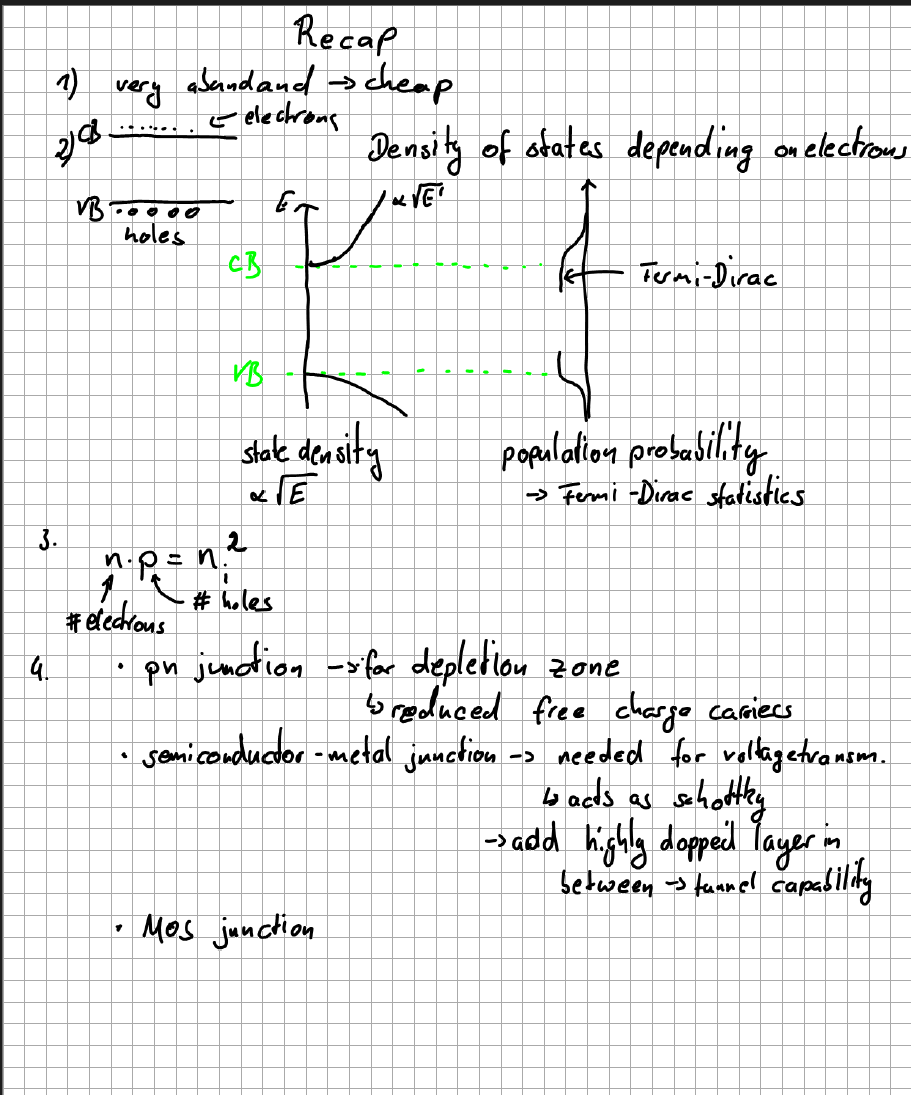
\includegraphics[width=3cm]{graphics/Meine_Mitschriften_Tablet.png}};
        \pause
        \node[anchor=south east] at ([shift={(-1.5cm,2cm)}]current page.south east) {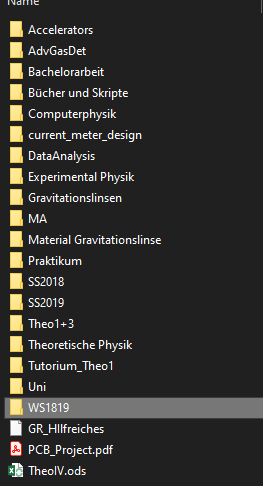
\includegraphics[width=3cm]{graphics/Meine-Unterlagen.png}};
        \pause
        \node[anchor=south east] at ([shift={(-2.5cm,4cm)}]current page.south east) {
\includegraphics[height=4cm]{graphics/overwhelmed_student_2.jpg}};
    \end{tikzpicture}
    \pause
    \vspace{1cm}
\end{frame}

\note{
        \begin{itemize}
            \item Welche Formate eignen sich für meine Notizen?
            \item Wie organisiere ich meine Notizen so, dass ich nicht im Chaos versinke?
            \item Wie kann ich mit meinen Komilitonen zusammenarbeiten und unterlagen teilen?
        \end{itemize}
    }